\documentclass{article}
\usepackage{iclr2026_conference,times}
\input{math_commands.tex}
\usepackage{hyperref}
\usepackage{url}
\usepackage{booktabs}
\usepackage{graphicx}
\title{Contact Topology World Models Do Not Improve MuJoCo Contact-Chain Control}
\author{Anonymous Authors}
\begin{document}
\maketitle

\begin{abstract}
We rebuilt a generated robotics idea into a concrete contact-rich manipulation study: should world models predict contact graph topology changes rather than only state trajectories?  The v4 rebuild implements a MuJoCo tabletop benchmark with a pusher, two movable blocks, walls, a fixture, and a target pocket.  It logs contact edges, births/deaths, graph edit distance, components, jam/safety events, task progress, seven random seeds, uncertainty intervals, paired statistics, ablations, stress sweeps, and negative cases.  The result is negative.  On the decisive combined-stress split, the proposed \texttt{topology\_world\_model} reaches $0.107 \pm 0.083$ task success, while the strongest non-oracle baseline, \texttt{ensemble\_uncertainty\_planner}, reaches $0.125 \pm 0.076$.  The paired success difference is $-0.018 \pm 0.035$.  The topology model improves edge F1 over that ensemble baseline, but does not convert graph prediction into better control.  We therefore mark the paper \textbf{KILL/ARCHIVE} for ICLR main.
\end{abstract}

\section{Decision}
This document is the v4 ICLR-main gate for Paper 73, \emph{Contact Topology World Models}.  The previous version was killed because it had only a synthetic template.  The current rebuild adds a real local MuJoCo benchmark and implemented baselines.  The rejection reason has changed: the evidence now exists, but it does not support the central claim.

\section{Hypothesis}
The tested hypothesis is that explicitly predicting contact graph topology changes, including contact births/deaths, connected components, and jam modes, improves contact-rich action selection beyond state-only dynamics, distance thresholds, pairwise contact classifiers, uncertainty ensembles, and contact-implicit control.  For the paper to become submission-relevant, topology prediction must improve downstream task success, not only an intermediate graph metric.

\section{Benchmark}
The benchmark uses MuJoCo dynamics for a planar pusher, two sliding blocks, static walls, a movable fixture, and a pocket.  The task is to create a useful pusher-block-block-pocket contact chain without jamming against the fixture or walls.  Five evaluation splits are used: nominal push-to-pocket, contact-chain transfer, fixture topology shift, friction/mass shift, and combined stress.  Combined stress includes fixture shift, friction/mass shift, contact-sensor noise, actuator limits, and distractor contacts.

The main evaluation contains 2240 rollouts: 5 splits, 7 seeds, 8 episodes per seed/split, and 8 methods.  The ablation study contains 252 rollouts.  The stress sweep contains 1050 rollouts.  All intervals are 95 percent confidence intervals over seed-level means.

\section{Methods}
The implemented methods are:
\begin{itemize}
\item \texttt{last\_contact\_persistence}: predicts the next graph from the previous graph.
\item \texttt{distance\_threshold\_graph}: predicts contacts from pairwise distances and relative geometry.
\item \texttt{state\_only\_dynamics\_model}: predicts state deltas and induces contacts from predicted state.
\item \texttt{pairwise\_contact\_classifier}: supervised pairwise contact predictor.
\item \texttt{ensemble\_uncertainty\_planner}: conservative ensemble over pairwise/topology predictors.
\item \texttt{contact\_implicit\_mpc\_baseline}: geometric contact-implicit controller with contact-distance penalties.
\item \texttt{topology\_world\_model}: proposed contact graph transition predictor and topology-aware planner.
\item \texttt{oracle\_topology\_planner}: upper bound with true next topology for prediction metrics.
\end{itemize}

\section{Main Results}
Table~\ref{tab:main} shows the combined-stress result.  The topology model has lower safety violations than several baselines and higher edge F1 than the uncertainty ensemble, but it does not win on task success.

\begin{table}[h]
\centering
\small
\begin{tabular}{lccccc}
\toprule
Method & Success & Edge F1 & Graph edit & Safety & Progress \\
\midrule
\texttt{oracle\_topology\_planner} & $0.250 \pm 0.076$ & 1.000 & 0.000 & 0.000 & 0.707 \\
\texttt{ensemble\_uncertainty\_planner} & $0.125 \pm 0.076$ & 0.364 & 0.276 & 0.237 & 0.649 \\
\texttt{contact\_implicit\_mpc\_baseline} & $0.107 \pm 0.083$ & 0.861 & 0.059 & 0.283 & 0.583 \\
\texttt{distance\_threshold\_graph} & $0.107 \pm 0.083$ & 0.871 & 0.055 & 0.285 & 0.581 \\
\texttt{last\_contact\_persistence} & $0.107 \pm 0.083$ & 0.860 & 0.053 & 0.311 & 0.609 \\
\texttt{pairwise\_contact\_classifier} & $0.107 \pm 0.083$ & 0.541 & 0.235 & 0.270 & 0.665 \\
\texttt{state\_only\_dynamics\_model} & $0.107 \pm 0.083$ & 0.904 & 0.043 & 0.297 & 0.596 \\
\texttt{topology\_world\_model} & $0.107 \pm 0.083$ & 0.610 & 0.209 & 0.158 & 0.716 \\
\bottomrule
\end{tabular}
\caption{Combined-stress results.  Success is the downstream task criterion.  Edge F1 and graph edit are intermediate topology diagnostics.}
\label{tab:main}
\end{table}

The strongest non-oracle success baseline is \texttt{ensemble\_uncertainty\_planner}.  The paired topology-minus-ensemble success difference is $-0.018 \pm 0.035$.  This fails the submission gate.  The result is especially instructive because the topology model improves edge F1 relative to the ensemble baseline but does not improve success.

\begin{figure}[h]
\centering
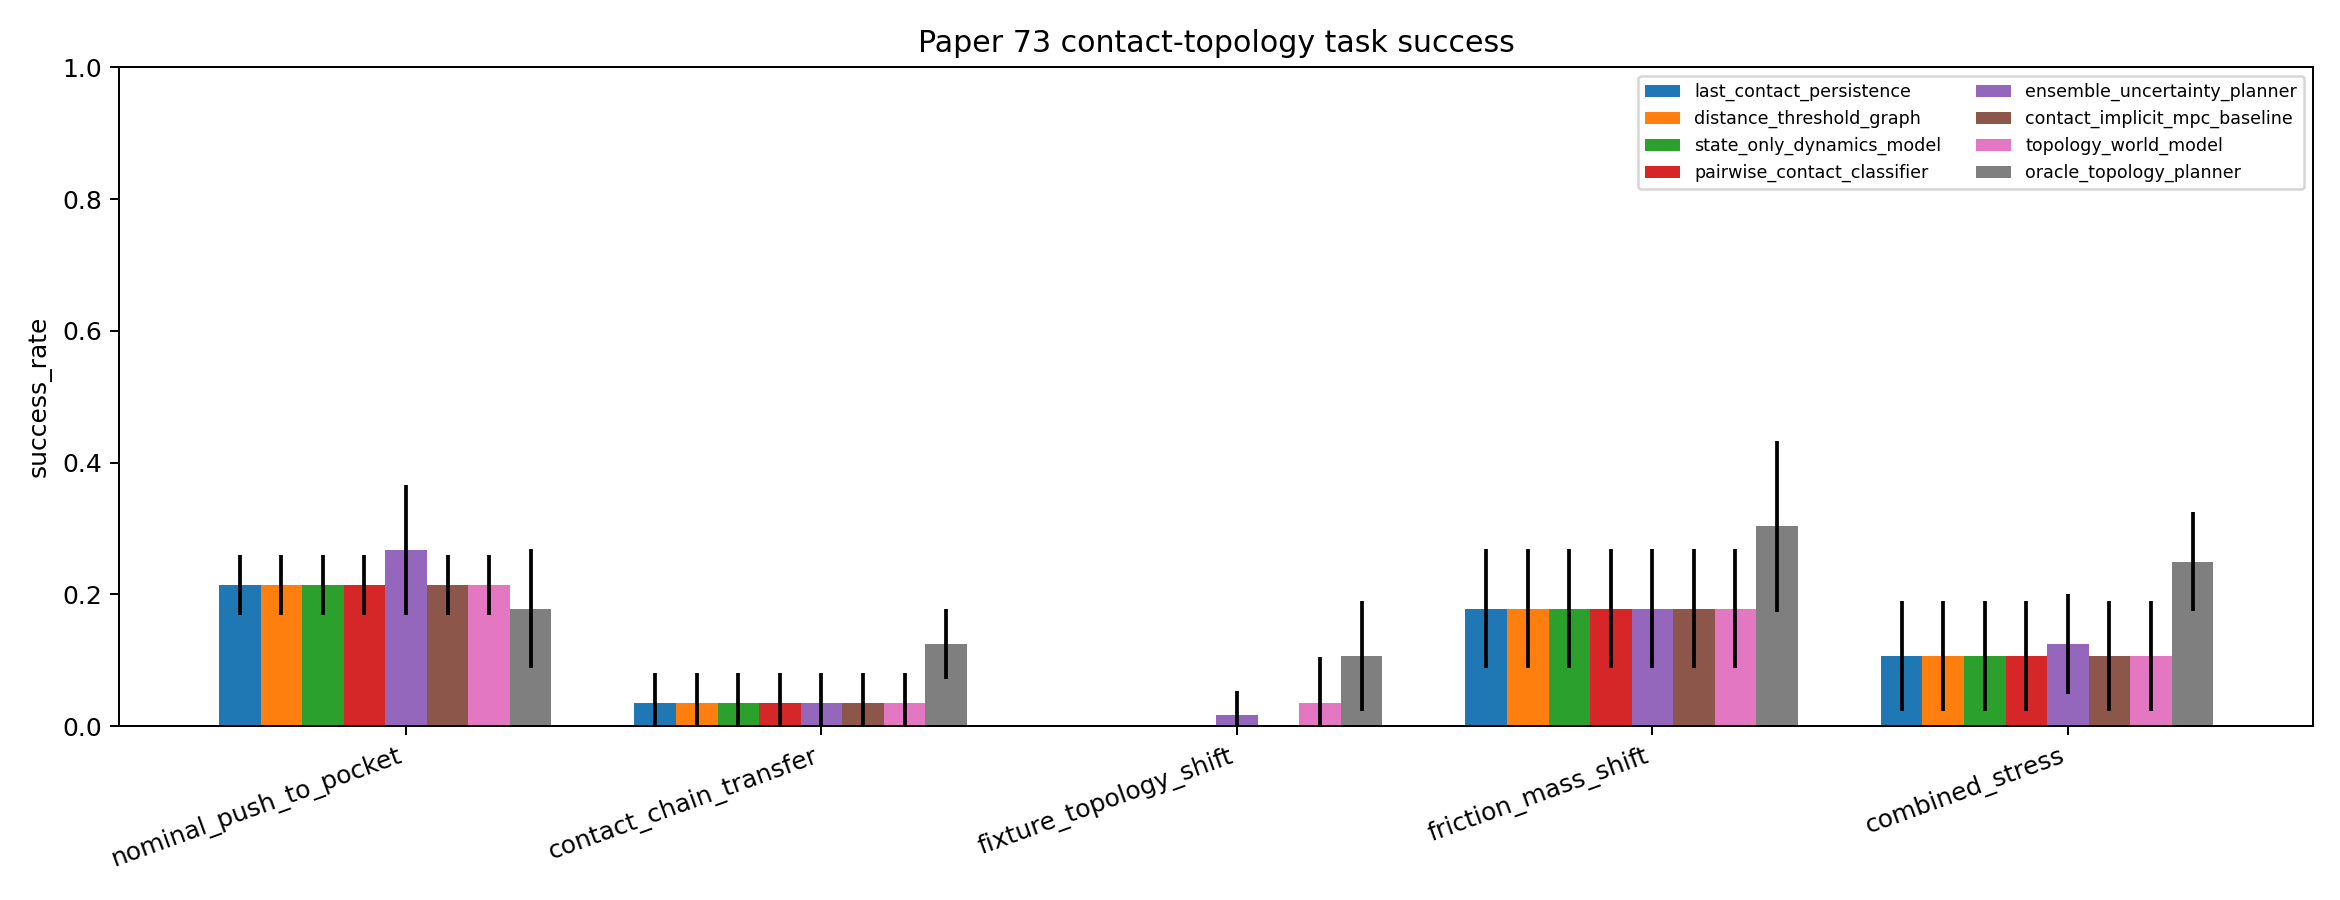
\includegraphics[width=0.95\linewidth]{../figures/topology_success_by_split.png}
\caption{Task success by split.  The topology model does not produce a decisive downstream success advantage.}
\end{figure}

\section{Ablations}
Table~\ref{tab:ablation} shows that topology-specific ablations are statistically overlapping.  Removing the uncertainty penalty slightly improves mean success, while the full model does not separate from no-birth/death, no-component, or no-jam variants.  The mechanism is therefore not supported.

\begin{table}[h]
\centering
\small
\begin{tabular}{lcccc}
\toprule
Ablation & Success & Edge F1 & Graph edit & Safety \\
\midrule
\texttt{topology\_no\_uncertainty\_penalty} & $0.095 \pm 0.097$ & 0.590 & 0.221 & 0.116 \\
\texttt{topology\_full} & $0.071 \pm 0.097$ & 0.583 & 0.220 & 0.081 \\
\texttt{topology\_no\_birth\_death} & $0.071 \pm 0.097$ & 0.569 & 0.224 & 0.170 \\
\texttt{topology\_no\_component\_head} & $0.071 \pm 0.097$ & 0.589 & 0.218 & 0.081 \\
\texttt{topology\_no\_jam\_slip} & $0.071 \pm 0.097$ & 0.554 & 0.225 & 0.061 \\
\texttt{topology\_no\_topology\_planner} & $0.071 \pm 0.097$ & 0.598 & 0.213 & 0.230 \\
\bottomrule
\end{tabular}
\caption{Combined-stress ablations.  No topology component produces a decisive task-success gain.}
\label{tab:ablation}
\end{table}

\section{Stress Sweep and Negative Cases}
The stress sweep shows the same pattern: topology sometimes improves graph diagnostics but does not dominate task success.  The oracle remains far from perfect at high stress, which means the local benchmark is hard but not yet a polished external benchmark contribution.  Negative cases concentrate around fixture-induced graph changes and wall/fixture jams where the topology predictor identifies contacts but the planner still chooses poor contact chains.

\begin{figure}[h]
\centering
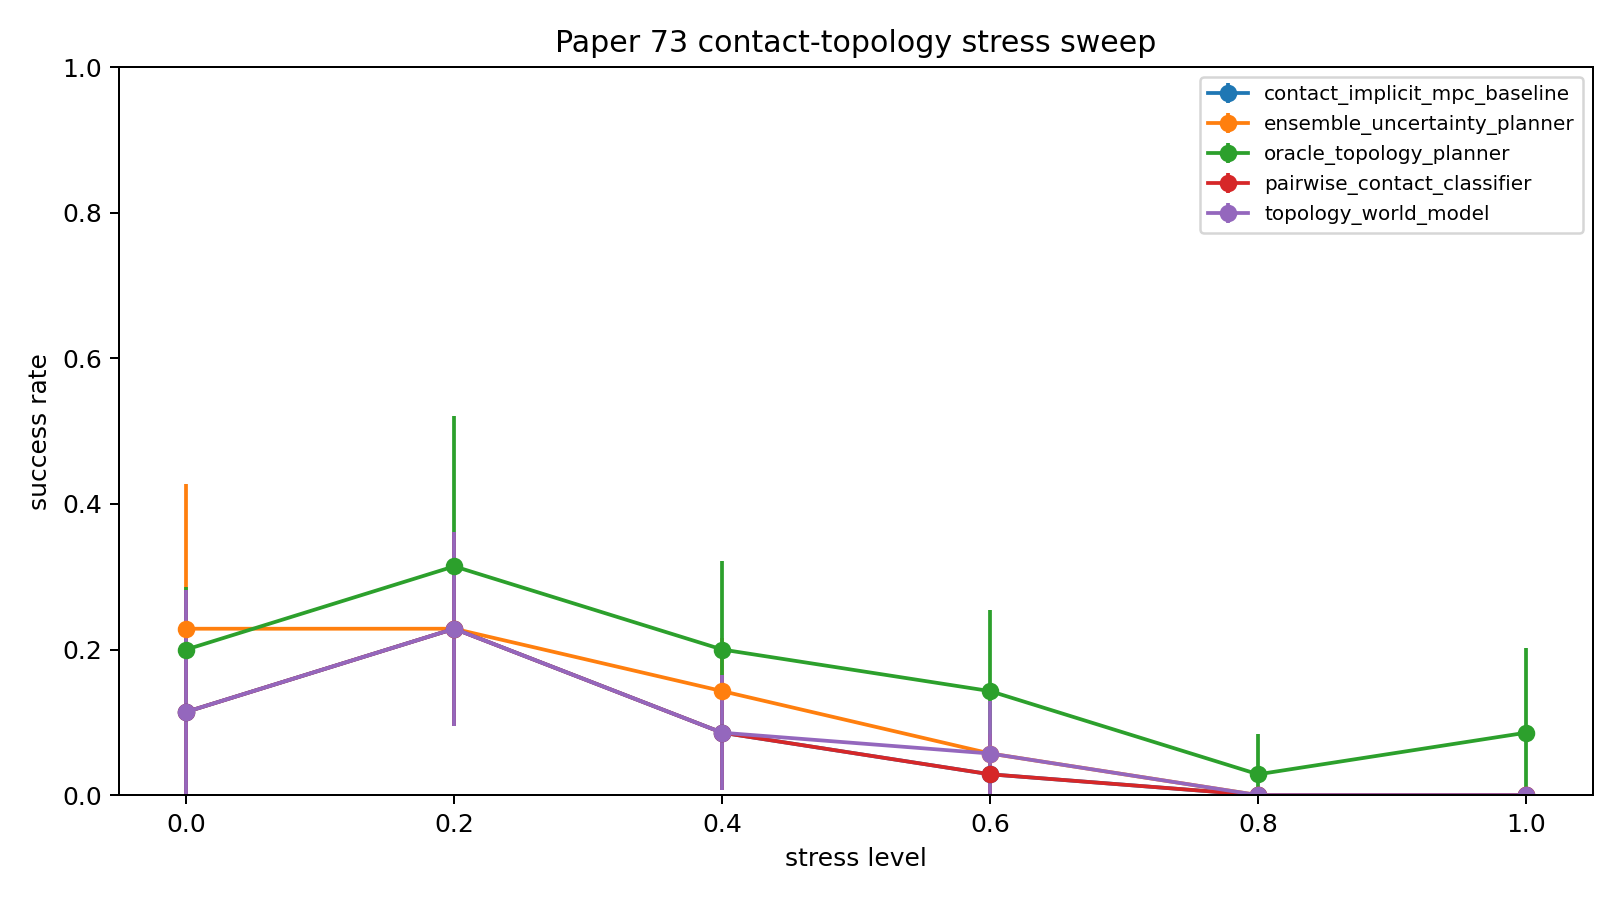
\includegraphics[width=0.82\linewidth]{../figures/topology_stress_sweep.png}
\caption{Stress sweep success.  The topology model does not dominate the strongest non-oracle baselines.}
\end{figure}

\section{Related Work Pressure}
The hostile prior-work set is crowded.  Visuotactile world modeling \citep{prior1}, robustness studies for world-action models \citep{prior2}, tactile/diffusion contact-rich policies \citep{prior3}, contact-implicit MPC \citep{prior4}, hybrid force-position policies \citep{prior5,prior6}, and adaptive contact-rich assembly \citep{prior7} all put pressure on the novelty boundary.  In this context, a contact-topology representation must deliver downstream gains.  It does not in the current evidence.

\section{Limitations}
This rebuild is not a real robot paper.  It lacks hardware experiments, videos, public benchmark validation, and a learned topology model trained on large contact-rich datasets.  The local MuJoCo benchmark is simplified and the oracle success rate is low, indicating that task calibration remains imperfect.  These limitations would matter even if the method won; because it does not win, they reinforce the archive decision.

\section{Conclusion}
Paper 73 should not be submitted to ICLR main.  The v4 rebuild provides useful evidence, but the evidence is negative: contact-topology prediction improves some graph metrics without improving downstream contact-chain control.  The correct terminal state is \textbf{KILL/ARCHIVE}.

\bibliographystyle{iclr2026_conference}
\bibliography{references}

\end{document}
